
\begin{enumerate}
    \item A student skates up a ramp that makes an angle \(30^\circ\) with the horizontal. He/she starts (as shown in the figure) at the bottom of the ramp with speed \(v_0\) and wants to turn around over a semicircular path \(xyz\) of radius \(R\) during which he/she reaches a maximum height \(h\) (at point \(y\)) from the ground as shown in the figure. Assume that the energy loss is negligible and the force required for this turn at the highest point is provided by his/her weight only. Then (\(g\) is the acceleration due to gravity)
        \begin{tasks}(2)
            \task \(v_0^2 - 2gh = \frac{1}{2}gR\)
            \task \(v_0^2 - 2gh = \frac{\sqrt{3}}{2}gR\)
            \task the centripetal force required at points \(x\) and \(z\) is zero
            \task the centripetal force required is maximum at points \(x\) and \(z\)
        \end{tasks}
    \begin{center}
        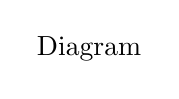
\begin{tikzpicture}
            \node {Diagram};
        \end{tikzpicture}
    \end{center}
\end{enumerate}
